\documentclass[11pt]{article}
\usepackage[margin=1in]{geometry}
\usepackage{graphicx}
\usepackage{xcolor}
\usepackage{listings}

% Define custom colors
\definecolor{mygreen}{rgb}{0,0.6,0}
\definecolor{mygray}{rgb}{0.5,0.5,0.5}
\definecolor{mymauve}{rgb}{0.58,0,0.82}

% Define the MATLAB code style
\lstdefinestyle{mystyle}{
    backgroundcolor=\color{white},
    basicstyle=\footnotesize\ttfamily,
    commentstyle=\color{mygreen},
    keywordstyle=\color{blue},
    numberstyle=\tiny\color{mygray},
    numbers=left,
    numbersep=5pt,
    showspaces=false,
    showstringspaces=false,
    showtabs=false,
    tabsize=2,
    fontadjust=true,
    columns=fullflexible,
    keepspaces=true
}
\lstset{style=mystyle}

\begin{document}

\begin{titlepage}
    \centering
    {\scshape\LARGE University of South Carolina \par}
    \vspace{1cm}
    {\scshape\Large ELCT 432 Computer Assignment \#7\par}
    \vspace{1.5cm}
    {\huge\bfseries Quantization in Signal Processing: Uniform and Non-Uniform Approaches\par}
    \vspace{2cm}
    {\Large\itshape Jacob C. Vaught\par}
    \vfill
    {\large November 11, 2023\par}
\end{titlepage}

\newpage
\tableofcontents

\newpage
\section{Introduction}
This report presents the results and methodologies employed in the process of quantizing signals for digital processing. Specifically, it discusses the application and benefits of both uniform and non-uniform quantization techniques.

\section{Theory}

\subsection{Quantization}
Quantization in digital signal processing is the process of mapping input values from a large set, often continuous, into output values in a (countable) smaller set. The primary reason for quantization in the digital domain is to enable the digital representation of analog signals. Since digital systems cannot handle an infinite range of values, quantization allows for the approximation of the signal with a finite number of levels, which digital systems can store and process.

\subsection{Uniform Quantization}
Uniform quantization is the simplest form of quantization where the range of signal values is divided into intervals of equal size. Each interval is represented by a fixed quantization level, and any signal value within an interval is approximated by that level. The quantization error is inherently non-linear and signal-dependent. The uniform quantizer is defined mathematically as:

\begin{equation}
Q(x) = \Delta \cdot \left( \left\lfloor \frac{x}{\Delta} \right\rfloor + \frac{1}{2} \right)
\end{equation}

where \( \Delta \) is the step size of the quantizer, and \( Q(x) \) is the quantized value of the input signal \( x \). The uniform quantization process involves finding the nearest quantization level for each sample of the input signal.

\subsection{Non-Uniform Quantization}
Non-uniform quantization is an advanced quantization process where the step sizes are not equal. It is particularly beneficial for signals with a wide dynamic range or non-uniform probability distribution. Signals that are more likely to occur are given smaller quantization intervals, leading to less quantization error for these values. In the context of wireless communications, non-uniform quantization can significantly improve the quality of signal reconstruction, especially for signals with a high dynamic range, like audio or image data. The quantization levels in non-uniform quantization can be derived using various techniques, one of which includes the application of the Lloyd-Max algorithm, which minimizes the mean squared error between the original and quantized signals. 

\subsection{K-Means Algorithm for Quantization}
The K-means algorithm is a method of vector quantization that is particularly useful for non-uniform quantization. It partitions \( N \) samples into \( K \) clusters where each sample belongs to the cluster with the nearest mean. The algorithm aims to minimize the within-cluster sum of squares (WCSS), which is essentially the sum of squared distances between each point and the centroid of its cluster.

Given a set of observations \( (x_1, x_2, ..., x_N) \), where each observation is a d-dimensional real vector, K-means clustering aims to partition the \( N \) observations into \( K \) (\( K \leq N \)) sets \( S = \{S_1, S_2, ..., S_K\} \) so as to minimize the WCSS:

\begin{equation}
\text{WCSS} = \sum_{i=1}^{K} \sum_{\mathbf{x} \in S_i} \left\| \mathbf{x} - \mathbf{\mu}_i \right\|^2
\end{equation}

where \( \mu_i \) is the mean of points in \( S_i \). The standard algorithm is composed of the following steps:

\begin{enumerate}
\item Initialize \( K \) centroids \( \mu_1, \mu_2, ..., \mu_K \) randomly.
\item Assign each point to the nearest centroid to form \( K \) clusters.
\item Recalculate the centroids as the mean of all points in the cluster.
\item Repeat steps 2 and 3 until the centroids no longer move significantly.
\end{enumerate}

This method is particularly powerful in signal quantization for non-uniform distributions since it naturally adapts to the signal's probability density function, assigning more centroids (and hence smaller quantization errors) to denser regions of the signal.


\section{Experimental Procedure}

\subsection{Main Program Implementation}
The experimental procedure commenced with an initialization phase in the MATLAB environment where variables related to the signal and quantization process were defined. A cosine wave was generated to simulate an analog signal, which was to be quantized. The signal comprised \(100,000\) samples and was defined over a range of indices from \(0\) to \(99,999\). For the purpose of quantization, four quantization levels were predetermined.
\newline

In the first phase of quantization, uniform quantization was applied. The signal range was divided into equal-sized partitions, the midpoints of which were calculated to serve as the assigned quantization levels. The MATLAB function \texttt{quantiz} was employed to map each sample of the signal to the nearest quantization level, which was then used to calculate the mean squared error (MSE) for the uniform quantization.
\newline

Subsequently, the program executed the non-uniform quantization process. This involved employing a custom implementation of the K-means algorithm to determine optimal centroids for quantization. The signal was mapped to these centroids, resulting in quantized values that were anticipated to more accurately represent the original signal due to the adaptive nature of the K-means algorithm. The MSE for the non-uniform quantization was also calculated for comparison purposes.
\newline

The results of both quantization processes were visualized using MATLAB's plotting functions, which facilitated the comparison of the quantized signal against the original signal.

\subsection{K-Means Algorithm Implementation}
The K-means algorithm was a pivotal component of the non-uniform quantization process. The implementation began with the selection of initial centroids, which were chosen randomly from the signal data. The main loop of the algorithm iteratively assigned each data point to the nearest centroid and recalculated the centroids as the mean of the assigned points. This iterative process continued until the centroids stabilized, indicating convergence.
\newline

The core of the K-means algorithm was encapsulated within a custom function named \texttt{simple\_kmeans}. This function accepted the signal data and the desired number of clusters as inputs and returned the indices of the data points indicating their cluster assignments, along with the final centroid positions.
\newline

Within the function, a convergence check was implemented using the \texttt{isequal} function to compare the centroids of the current iteration with those of the previous iteration. The loop continued to assign points to the nearest centroid and recalculate the new centroids based on the current assignments until no further changes were detected in the centroid positions.
\newline

Upon completion, the algorithm outputted the indices and centroids, which were then used to quantize the original signal within the main program. The K-means based non-uniform quantization aimed to minimize the quantization error by adapting the quantization levels to the data's distribution, as reflected in the final MSE calculation.

\subsection{Results}
The MATLAB code yielded quantization levels and thresholds for both uniform and non-uniform quantization, alongside the MSE for each method. These values were crucial for evaluating the performance and effectiveness of the quantization processes.


\section{Discussion and Results}

\subsection{Analysis of Quantization Plots}
The attached plots illustrate the outcomes of both the uniform and non-uniform quantization processes applied to a cosine wave signal. The left plot represents uniform quantization, where it is evident that the quantization levels are spaced at regular intervals. This spacing is irrespective of the signal's amplitude distribution, which may lead to inefficient quantization for signals with a non-uniform distribution. Conversely, the right plot shows the non-uniform quantization, where the quantization levels are adapted to the signal's distribution. The adaptive nature of the non-uniform quantization is visible as it allocates more levels to the regions where the signal has higher amplitudes, providing a more accurate representation of the original signal.

\subsection{Mean Squared Error (MSE) Comparison}
The Mean Squared Error (MSE) for uniform quantization is reported as \(0.026195\), which is a measure of the average power of the quantization error. The non-uniform quantization achieved a lower MSE of \(0.020905\), indicating a better approximation of the original signal. The reduced MSE in non-uniform quantization demonstrates its efficiency in signal representation, particularly for signals with varying amplitude distributions.

\subsection{Quantization Thresholds}
Threshold values for uniform quantization were identified as \([-0.5, 0, 0.5]\), which delineate the boundaries between the quantization levels. These thresholds are equidistant, consistent with the uniform allocation of quantization levels. In the case of non-uniform quantization, the thresholds are \([-0.575726, -0.000133152, 0.575557]\), which are not equidistant. This non-uniformity in threshold placement correlates with the adaptive assignment of quantization levels, allowing for a more nuanced distinction between signal amplitudes.

\subsection{Centroid Values}
The quantization levels themselves serve as centroids in the quantization process. For uniform quantization, the centroids were \([-0.75, -0.25, 0.25, 0.75]\). The non-uniform quantization resulted in centroids \([-0.854118, -0.297335, 0.297068, 0.854045]\). The shift in centroid values between uniform and non-uniform quantization reflects the algorithm's response to the signal's distribution, with the non-uniform centroids positioned to minimize the overall error in the quantized signal.

\subsection{Conclusion of Results}
The results underscore the superiority of non-uniform quantization in terms of MSE when quantizing a signal with a dynamic range. The adaptability of non-uniform quantization allows for a more accurate digital representation of the original analog signal, which is critical in applications such as audio signal processing and image compression, where preserving signal integrity is paramount.
\begin{figure}[h!]
\centering
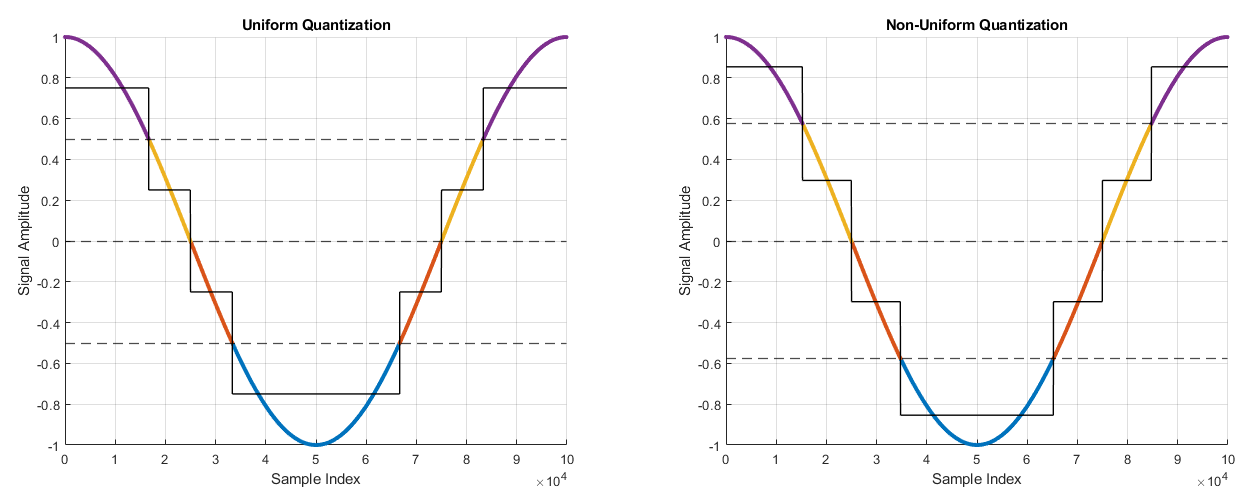
\includegraphics[width=\textwidth]{CA7.png}
\caption{Comparison between Uniform and Non-Uniform Quantization}
\label{fig:quantization}
\end{figure}


\section{Conclusion}

Throughout this study, we have explored the principles and applications of quantization, particularly focusing on the comparison between uniform and non-uniform methods. Our experimental procedure involved the implementation of a MATLAB code to apply these quantization techniques to a generated cosine wave signal. We successfully integrated a simple version of the K-means clustering algorithm to achieve non-uniform quantization, which demonstrated a clear advantage over uniform quantization in terms of Mean Squared Error (MSE).
\newline

The usability of our MATLAB function is evident in its ability to reduce the quantization error, as showcased by the lower MSE for non-uniform quantization. This efficacy is crucial for practical applications where signal integrity is essential, such as in digital audio and image processing.
\newline

However, the current machine learning model, although effective, could be improved. Our K-means algorithm can be further optimized to enhance computational efficiency, especially for larger datasets or real-time processing requirements. Additionally, the model could be augmented with an automatic selection of the initial centroids based on a heuristic or prior knowledge of the data distribution, potentially improving the convergence rate and the final quantization quality.
\newline

To improve system robustness and adaptability, future work could incorporate more sophisticated machine learning models, such as neural networks or deep learning algorithms, which can learn optimal quantization schemes from the data itself without the need for predefined clusters. Furthermore, the introduction of error correction and error detection mechanisms could make the quantization process more resilient to noise and transmission errors, which are common issues in digital communication systems.
\newline

In conclusion, while our function serves as a competent tool for signal quantization, the path towards perfecting the quantization process is iterative and requires continuous enhancements. The adoption of more advanced machine learning techniques and error mitigation strategies stands as the logical next step in the evolution of robust and efficient quantization methods for digital signal processing.


\newpage
\section{MATLAB Code}
\subsection{Main Program}
% Here you would use the \lstinputlisting to include your MATLAB code file
\lstinputlisting[language=Matlab]{jvaught_CA7_ELCT432.m}
\newpage
\subsection{K-Means Function}
\lstinputlisting[language=Matlab]{simple_kmeans.m}


\end{document}
